% --------------------------------------------------------------------------- %
% Poster for the 5th ACM International Symposium on Pervasive Displays        %
% Oulu, Finland                                                               %
% 20-22 June, 2016                                                            %
% --------------------------------------------------------------------------- %
%
% Poster template reference
% http://www.brian-amberg.de/uni/poster/
%
% --------------------------------------------------------------------------- %


\documentclass[a0paper,portrait]{baposter}

\usepackage{calc}
\usepackage{graphicx}
\usepackage{amsmath}
\usepackage{amssymb}
\usepackage{relsize}
\usepackage{multirow}
\usepackage{rotating}
\usepackage{bm}
\usepackage{url}

\usepackage{graphicx}
\usepackage{multicol}

\newcommand{\captionfont}{\footnotesize}

\graphicspath{{images/}{../images/}}
\usetikzlibrary{calc}

\newcommand{\SET}[1]  {\ensuremath{\mathcal{#1}}}
\newcommand{\MAT}[1]  {\ensuremath{\boldsymbol{#1}}}
\newcommand{\VEC}[1]  {\ensuremath{\boldsymbol{#1}}}
\newcommand{\Video}{\SET{V}}
\newcommand{\video}{\VEC{f}}
\newcommand{\track}{x}
\newcommand{\Track}{\SET T}
\newcommand{\LMs}{\SET L}
\newcommand{\lm}{l}
\newcommand{\PosE}{\SET P}
\newcommand{\posE}{\VEC p}
\newcommand{\negE}{\VEC n}
\newcommand{\NegE}{\SET N}
\newcommand{\Occluded}{\SET O}
\newcommand{\occluded}{o}


\usepackage[utf8]{inputenc}
%Ionuţ-Alexandru Zaiţi, Ştefan-Gheorghe Pentiuc, Radu-Daniel Vatavu
%http://www.latex-community.org/forum/viewtopic.php?f=31&t=9084


%%%%%%%%%%%%%%%%%%%%%%%%%%%%%%%%%%%%%%%%%%%%%%%%%%%%%%%%%%%%%%%%%%%%%%%%%%%%%%%%
%%%% Some math symbols used in the text
%%%%%%%%%%%%%%%%%%%%%%%%%%%%%%%%%%%%%%%%%%%%%%%%%%%%%%%%%%%%%%%%%%%%%%%%%%%%%%%%

%%%%%%%%%%%%%%%%%%%%%%%%%%%%%%%%%%%%%%%%%%%%%%%%%%%%%%%%%%%%%%%%%%%%%%%%%%%%%%%%
% Multicol Settings
%%%%%%%%%%%%%%%%%%%%%%%%%%%%%%%%%%%%%%%%%%%%%%%%%%%%%%%%%%%%%%%%%%%%%%%%%%%%%%%%
\setlength{\columnsep}{1.5em}
\setlength{\columnseprule}{0mm}

%%%%%%%%%%%%%%%%%%%%%%%%%%%%%%%%%%%%%%%%%%%%%%%%%%%%%%%%%%%%%%%%%%%%%%%%%%%%%%%%
% Save space in lists. Use this after the opening of the list
%%%%%%%%%%%%%%%%%%%%%%%%%%%%%%%%%%%%%%%%%%%%%%%%%%%%%%%%%%%%%%%%%%%%%%%%%%%%%%%%
\newcommand{\compresslist}{%
\setlength{\itemsep}{1pt}%
\setlength{\parskip}{0pt}%
\setlength{\parsep}{0pt}%
}

%%%%%%%%%%%%%%%%%%%%%%%%%%%%%%%%%%%%%%%%%%%%%%%%%%%%%%%%%%%%%%%%%%%%%%%%%%%%%%
%%% Begin of Document
%%%%%%%%%%%%%%%%%%%%%%%%%%%%%%%%%%%%%%%%%%%%%%%%%%%%%%%%%%%%%%%%%%%%%%%%%%%%%%

\begin{document}

%%%%%%%%%%%%%%%%%%%%%%%%%%%%%%%%%%%%%%%%%%%%%%%%%%%%%%%%%%%%%%%%%%%%%%%%%%%%%%
%%% Here starts the poster
%%%---------------------------------------------------------------------------
%%% Format it to your taste with the options
%%%%%%%%%%%%%%%%%%%%%%%%%%%%%%%%%%%%%%%%%%%%%%%%%%%%%%%%%%%%%%%%%%%%%%%%%%%%%%
% Define some colors

% \definecolor{lightblue}{cmyk}{0.83,0.24,0,0.12}
\definecolor{lightblue}{rgb}{0.145,0.6666,1}

\definecolor{bgc_1}{RGB}{93, 194,232}
\definecolor{bgc_2}{RGB}{144, 190, 242}


\definecolor{hc_1}{RGB}{29,105,218}
\definecolor{hc_2}{RGB}{240,141,96}


\hyphenation{perform repetitions comfortable provides recognition triaxial}

%%
\begin{poster}%
  % Poster Options
  {
  % Show grid to help with alignment
  grid=false,
  % Column spacing
  colspacing=1em,
  % Color style
  bgColorOne=white,
  bgColorTwo=white,
  borderColor=lightblue,
  headerColorOne=black,
  headerColorTwo=lightblue,
  headerFontColor=white,
  boxColorOne=white,
  boxColorTwo=lightblue,
  % Format of textbox
  textborder=roundedleft,
  % Format of text header
  eyecatcher=true,
  headerborder=closed,
  headerheight=0.125\textheight,
%  textfont=\sc, An example of changing the text font
  headershape=roundedright,
  headershade=shadelr,
  headerfont=\Large\bf\textsc, %Sans Serif
  textfont={\setlength{\parindent}{1.5em}},
  boxshade=plain,
%  background=shade-tb,
  background=plain,
  linewidth=2pt
  }
%%% Eye Cacther %%%%%%%%%%%%%%%%%%%%%%%%%%%%%%%%%%%%%%%%%%%%%%%%%%%%%%%%%%%%%%%
{
	Eye Catcher, empty if option eyecatcher=false - unused
%    
\includegraphics[height=3em]{conacyt_logo_v1.png}
}
%%% Title %%%%%%%%%%%%%%%%%%%%%%%%%%%%%%%%%%%%%%%%%%%%%%%%%%%%%%%%%%%%%%%%%%%%%
{\bf
  {Understanding Movement Variability of \\ Simplistic Gestures Using an Inertial Sensor}
}
%%% Authors %%%%%%%%%%%%%%%%%%%%%%%%%%%%%%%%%%%%%%%%%%%%%%%%%%%%%%%%%%%%%%%%%%%
{
	%\vspace{-0.3em} 
	{\smaller {Miguel Xochicale\textsuperscript{1}, Chris Baber\textsuperscript{1} and Mourad Oussalah\textsuperscript{2}}; [map479@bham.ac.uk]  } \\ 
	%\vspace{-0.5em}
	{\smaller
	\textsuperscript{1} School of Electronic, Electrical and Systems Engineering, University of Birmingham, UK \\
	\textsuperscript{2} Center for Ubiquitous Computing, University of Oulu, Finland }
}
% Logos
  {% The makebox allows the title to flow into the logo, this is a hack because of the L shaped logo.
  	\fbox{
    \begin{minipage}{11em}
    
      \begin{center}
      
\includegraphics[height=2.7em]{conacyt_logo_v1}\\
      
\includegraphics[height=2.95em]{uob_logo} \\
      
\includegraphics[height=1.8em]{University_of_Oulu_logo}  
      \end{center}
      
    \end{minipage}
      }
  } 


%%%%%%%%%%%%%%%%%%%%%%%%%%%%%%%%%%%%%%%%%%%%%%%%%%%%%%%%%%%%%%%%%%%%%%%%%%%%%%
%%% Now define the boxes that make up the poster
%%%---------------------------------------------------------------------------
%%% Each box has a name and can be placed absolutely or relatively.
%%% The only inconvenience is that you can only specify a relative position 
%%% towards an already declared box. So if you have a box attached to the 
%%% bottom, one to the top and a third one which should be in between, you 
%%% have to specify the top and bottom boxes before you specify the middle 
%%% box.
%%%%%%%%%%%%%%%%%%%%%%%%%%%%%%%%%%%%%%%%%%%%%%%%%%%%%%%%%%%%%%%%%%%%%%%%%%%%%%
    %
    % A coloured circle useful as a bullet with an adjustably strong filling
    \newcommand{\colouredcircle}{%
      \tikz{\useasboundingbox (-0.2em,-0.32em) rectangle(0.2em,0.32em); 
      \draw[draw=black,fill=lightblue,line width=0.03em] (0,0) circle(0.18em);}}

      
      
      
\headerbox{Introduction}{name=problem,span=2,column=0,row=0}{

Variability is an inherent characteristic of human movement \cite{newell93}.
Generally, humans perform the same action slightly differently trial by trial
which is a common challenge in Human Activity Recogtion (HAR) \cite{bulling2014}.
The time-delay embedding theorem and Principal Component Analysis (PCA) have proven to be
reliable methods for feature extraction in HAR \cite{frank10, sama13}. 
It is therefore hypothesised that these methods might be useful to learn 
the variability of human activities. 
Therefore, the following research questions will be addressed: 

\begin{itemize}
\item Can we use the movement variability 
 not only to identify an activity but also to use it 
 as a index of user's performance
 over the course of training, practice or rehabilitation?
 
  \item How can the time-delay embedding and PCA methods quantify the variability of human activities?
\end{itemize}



% We belive that this prelimary study can give insight into the variability
% For these reasons we are interested in studying methods that can give insight 
% into the variability between individuals and repetitions of the same movement. 
% We believe that this preliminary study might provide useful information for 
% activity recognition, e.g. in terms of detecting changes 
% of user's behaviour (enthusiasm, boredom, tiredness or confusion) in 
% the way in which activities are performed over the course of training, 
% practice or rehabilitation.
}


\headerbox{Human Activity Recognition Chain}{name=arc,span=2,column=0,below=problem}{

Bulling \emph{et al.} \cite{bulling2014}, for instance, reviewed the state-of-the-art of
Human Activity Recognition to identify activities or gestures from body-worn intertial sensors.


\begin{center}
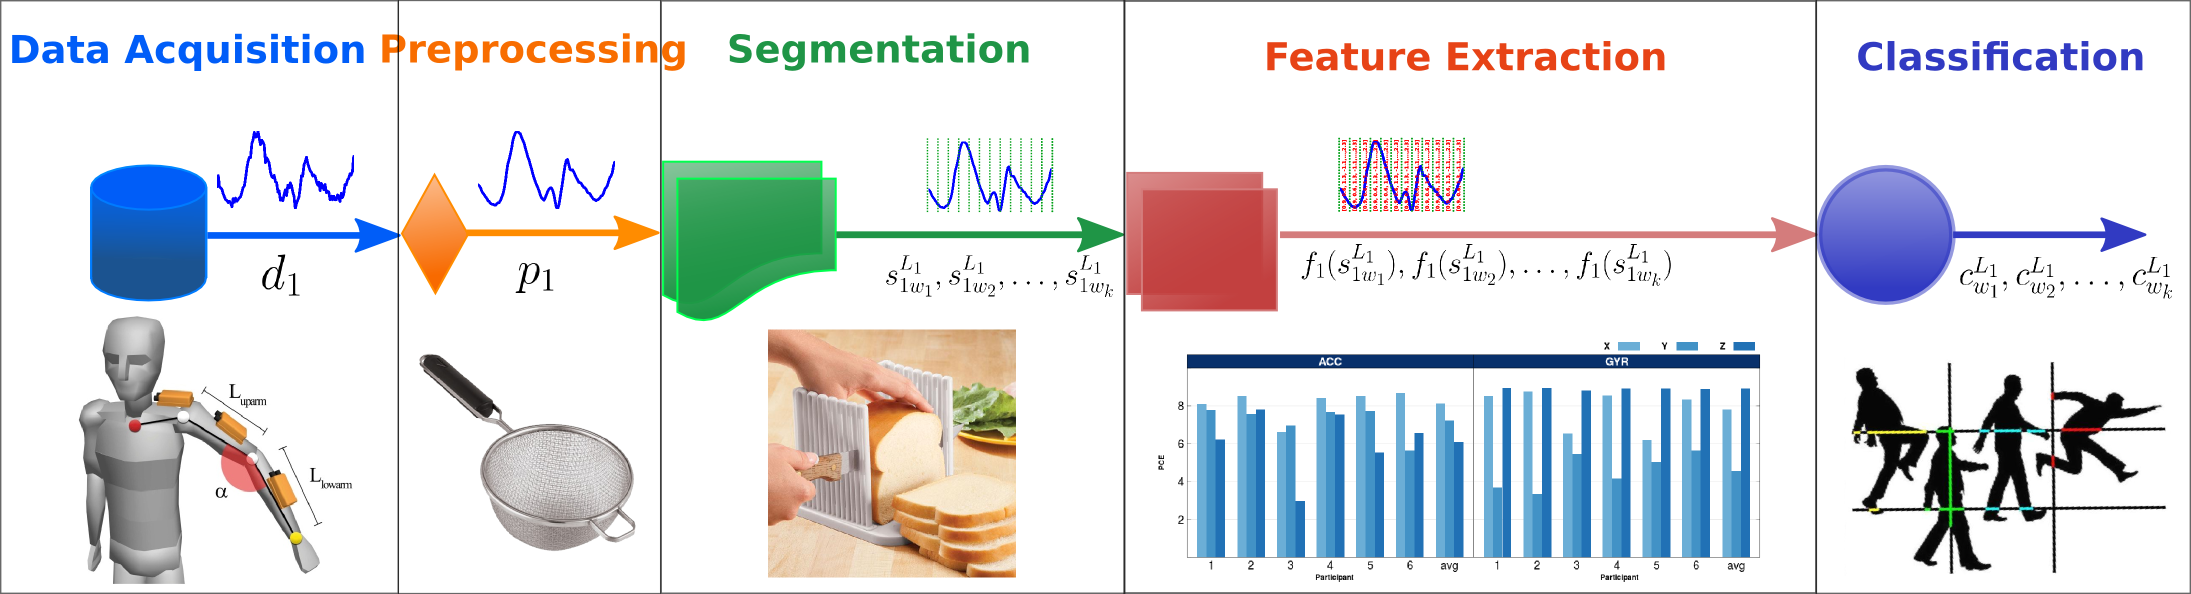
\includegraphics[width=1.0\textwidth]{arc02} 
\end{center}

Diagram is replicated from the work of Ban\~os \emph{et al.} \cite{banos2014}.
}

\headerbox{Materials and Methods}{name=methods,span=2,column=0,below=arc}{

Raw time-series data is collected from a triaxial accelerometer ($a_x, a_y, a_z$).
Then, a $N$ samples length time-series, e.g. $a_x$, is used to obtain the
time-delay embedded matrix, $E \{ a_x \}$, with $m=20$ and $\tau=6$ \cite{frank10, sama13}.
Finally, PCA is applied to  $E \{ a_x \}$ to compute 
the percentage of cumulative energy (PCE) \cite{nhammerla11}.




\begin{center}
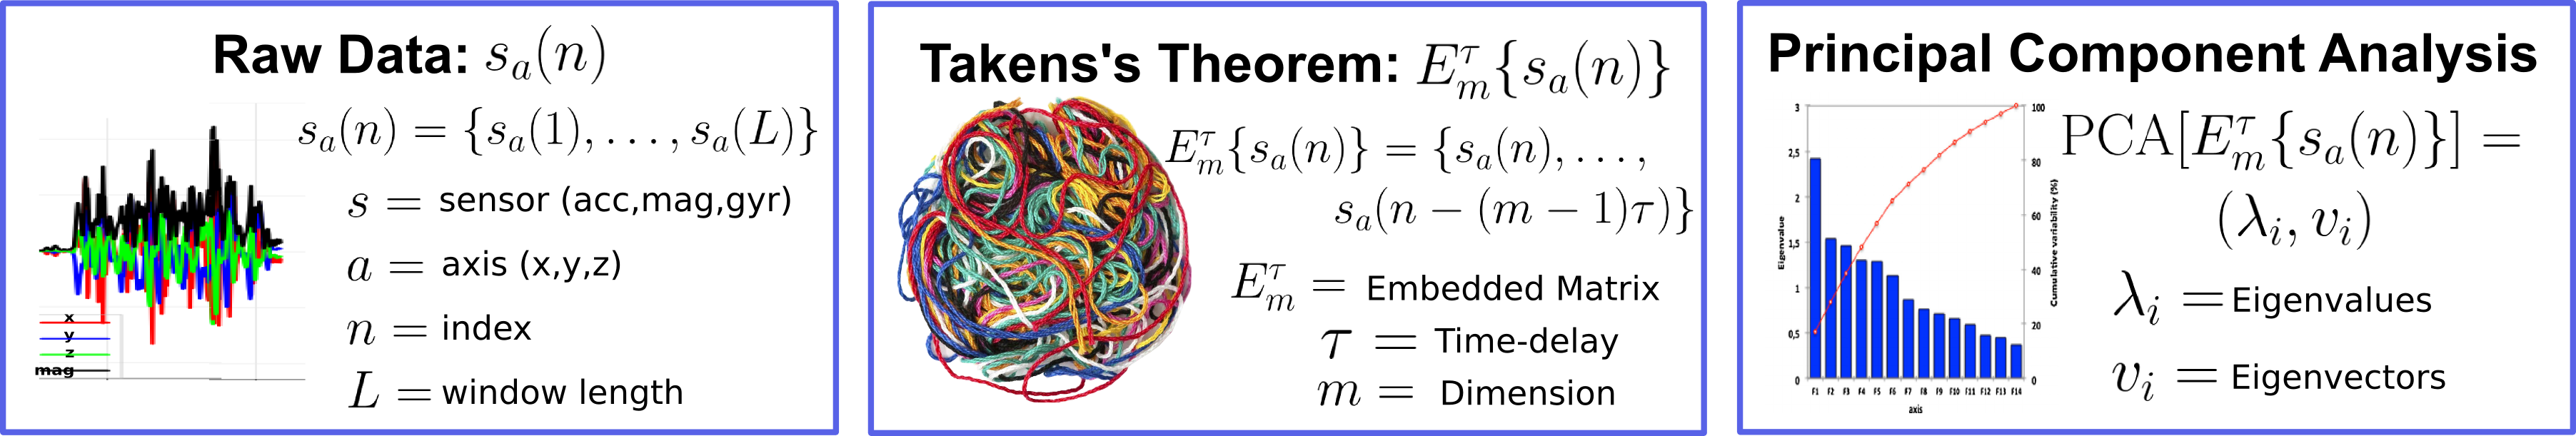
\includegraphics[width=1\linewidth]{method_diagram01} 
\end{center}


The method is then applied to six simple movements 
which were performed by five participants wearing a low-cost and commertial intertial sensor on their right wrist; 
each movement was continuously repeated for 10 seconds.

}

\headerbox{Conclusion and Outlook}{name=conclusion,span=2,column=0,below=methods}{

% Measuring variability in human activity
% offers an approach to understand user's performence over the course of training, 
% practice or rehabilitation.

Although the time-delay embedding technique is subject to different values of embedded parameters 
( $m$ and $\tau$ ) according to the length and complexity of the time-series,
the technique is useful to present the inherent features of
variability between five participants for six different
gestures.

In the future, we will collect data from a wider range of individuals
(gender and age) and from additional sensors.
Also, different classification techniques will be explored.
}

  
%%%%%%%%%%%%%%%%%%%%%%%%%%%%%%%%%%%%%%%%%%%%%%%%%%%%%%%%%%%%%%%%%%%%%%%%%%%%%%
\headerbox{References}{name=references,span=2,column=0,below=conclusion,above=bottom}{
%%%%%%%%%%%%%%%%%%%%%%%%%%%%%%%%%%%%%%%%%%%%%%%%%%%%%%%%%%%%%%%%%%%%%%%%%%%%%%
     \smaller
    \vspace{-0.4em} % Save some space at the beginning
    \bibliographystyle{ieee}
    \renewcommand{\section}[2]{\vskip 0.05em}

\begin{thebibliography}{1}
\itemsep=-0.01em
\setlength{\baselineskip}{0.4em}

\bibitem{newell93}
  Karl M. Newell and Daniel M. Corcos. 1993.
  \newblock Variability and motor control.
  \newblock Human Kinetics Publishers.
  
  
\bibitem{bulling2014}
  Andreas Bulling, Ulf Blanke and Bernt Schiele. 2014.
  \newblock A tutorial on human activity recognition using body-worn inertial sensors
  \newblock In {\em ACM Computing Surveys (CSUR)}, vol. 6, 1-33.
  
  \bibitem{frank10}
  Jordan Frank, Shie Mannor and Doina Precup. 2010. 
  \newblock Activity and Gait Recognition with Time-Delay Embeddings.
  \newblock In {\em Proceedings of the 24-th AAAI Conference on Artificial Intelligence}, 1581-1586.
  
\bibitem{sama13}
  Albert Samà, Francisco J. Ruiz, Núria Agell, Carlos Pérez-López, Andreu Català and Joan Cabestany. 2013.
  \newblock Gait identification by means of box approximation geometry of reconstructed attractors in latent space.
  \newblock In {\em Neurocomputing}, vol. 121, 79-88.

  
 
\bibitem{banos2014}
   Oresti Banos, Juan-Manuel Galvez, Miguel Damas, Hector Pomares and , Ignacio Rojas. 2014.
   \newblock Window size impact in human activity recognition.
   \newblock In {\em Sensors (Basel, Switzerland)}, 14, 6474-99

   
% \bibitem{figo10}
%   Davide Figo, Pedro C. Diniz, Diogo R. Ferreira and João M. P. Cardoso. 2010.
%   \newblock Preprocessing techniques for context recognition from accelerometer data.
%   \newblock In {\em Personal and Ubiquitous Computing}, vol. 7, 645-662.
%   
  

  
\bibitem{nhammerla11}
  Nils Y Hammerla, Thomas Plötz, Peter Andras and Patrick Olivier. 2011.
  \newblock Assessing Motor Performance with pca.
  \newblock In {\em International Workshop on Frontiers in Activity Recognition using Pervasive Sensing}, 18-23.

 

\end{thebibliography}
}


%,above=bottom
\headerbox{Results}{name=results,span=1,column=2,row=0,aligned=problem}{

The values of the percentage of cumulative energy (PCE) from five participants 
are presented using boxplots for both low-cost and commertial triaxial accelerometer (ACC) sensors.
It is evident that both sensors present similar results for each movement.
It is highlighted that the circular movement shows the least variation of ACC 
per component compare to the other movements. 

However, 
we assume that the evident variability of the movements 
is due to the flexibility in the experiment where participants
were only asked to perform the movements at a comfortable speed.


\vspace{-4mm}
\begin{center}
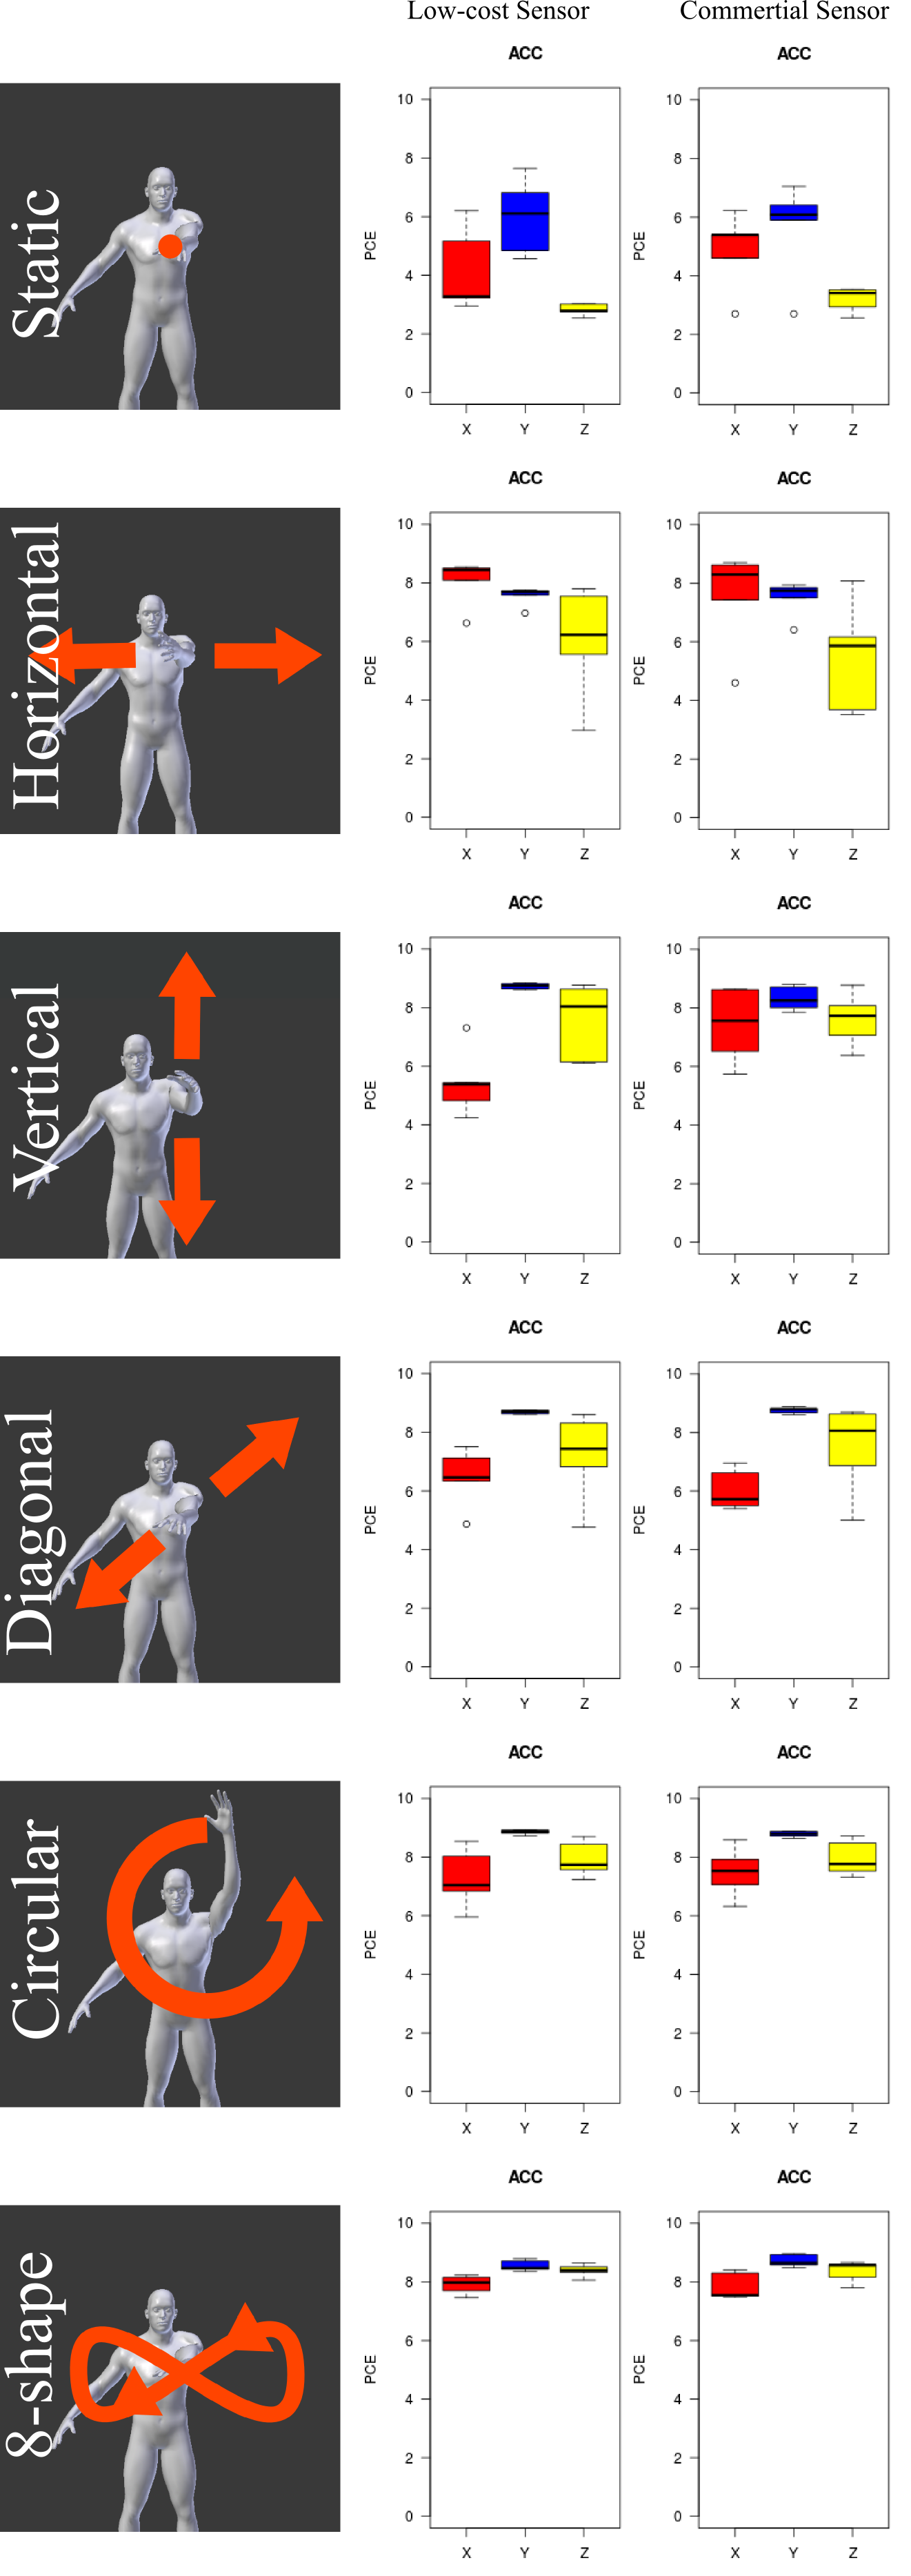
\includegraphics[width=0.94\linewidth]{movements_boxplot_07} 
\end{center}


}


\headerbox{Acknowledments}{name=acknowledments,span=1,column=2,row=0,above=bottom}{

Miguel Xochicale gratefully acknowledges the studentship 
from the National Council for Science and Technology (CONACyT) Mexico for pursuing his doctoral
studies at The University of Birmingham, UK.
}


  

\end{poster}

\end{document}
